%\documentclass[11pt,reqno]{amsart}
\documentclass[11pt,reqno]{article}
\usepackage[utf8]{inputenc}
\usepackage[brazil]{babel}
\usepackage{verbatim}

\usepackage{latexsym,amsmath}
%\usepackage[left=3cm,top=2.5cm,right=3cm,bottom=2.5cm]{geometry}
\usepackage[left=2.9cm,top=3.3cm,right=2.9cm,bottom=2.5cm]{geometry}
\usepackage{color}
\usepackage{amsthm}
\usepackage{amssymb}
\usepackage{epsfig}


\begin{document}

\pagestyle{empty}
\newtheorem{theorem}{Teorema}[section]
\newtheorem{cor}[theorem]{Corolário}
\newtheorem{lemma}[theorem]{Lema}
\newtheorem{fact}[theorem]{Fato}
\newtheorem{property}[theorem]{Propriedade}
\newtheorem{proposition}[theorem]{Proposição}
\newtheorem{definition}[theorem]{Definição}
\newtheorem{setup}[theorem]{Configuração}
\newtheorem{conjecture}[theorem]{Conjectura}

\theoremstyle{definition}
\newtheorem{example}[theorem]{Exemplo}
\newcommand\eps{\varepsilon}

\title{Estudo de coalisões em MAW}

\begin{comment}
\author[N. A. Martins]{Nicolas A. Martins}
\address{Departamento de Computação, Centro de Ciências, UFC --
  Campus do Pici, Bloco 910, 60455--760 Fortaleza, CE, Brazil} \email{\tt nicolasam@lia.ufc.br}

\author[S. S. J. Oliveira]{Samuel Oliveira}
\address{Departamento de Computação, Centro de Ciências, UFC --
  Campus do Pici, Bloco 910, 60455--760 Fortaleza, CE, Brazil} \email{\tt samuelservulo@lia.ufc.br}
\end{comment}

\author{
N. Martins, S. Oliveira \vspace{15pt}\\
Departamento de Computação, Universidade Federal do Ceará\\
Campus do Pici, Bloco 910, 60455--760 Fortaleza, CE, Brazil \vspace{10pt}\\
{\small {\tt \{nicolasam,samuelservulo\}@lia.ufc.br}}
}

\date{}

\maketitle
\thispagestyle{empty}

\begin{abstract}
MAW (Multi-Agent Wumpus) é um modelo adaptado do mundo de Wumpus \cite{russel03} para um sistema multi-agente. Neste artigo estudamos a formação de
coalisões no modelo adaptado  para três tipos fixos de agentes, com diferentes taxas de adesão,e verificamos os critérios de payoff individual de acordo com
 a coalisão formada.
\vspace{1pt}\\
{\bf PALAVRAS-CHAVE: coalisão, jogo competitivo/cooperativo.\\ÁREA: Sistemas Multi-agentes.}\\
\end{abstract}


\section{Introdução - o mundo de Wumpus}

O mundo de Wumpus [Russel et al, 2003] é um ambiente representado por um tabuleiro MxM com as seguintes características:
\begin{itemize}
\item[i.] Parcialmente observável;
\item[ii.] Determinístico;
\item[iii.] Episódico;
\item[iv.] Estático;
\item[v.] Discreto;
\item[vi.] Single-agent;
\end{itemize}


O mundo é composto por:

\begin{itemize}
\item[i.] Ouro, localizado em alguma posição do tabuleiro;
\item[ii.] Um agente, que deseja achar o tesouro;
\item[iii.] Um monstro, o Wumpus, que pode matar o agente;
\item[iv.] Buracos, onde o agente ou o Wumpus pode cair;
\end{itemize}

Claramente, é possível observar que os únicos modos de um agente morrer é caso caia num buraco ou o Wumpus o ache, fora estes dois casos.\\
O agente inicia numa posição específica do tabuleiro (a entrada para o mundo, normalmente a posição [1,1]) e deseja achar o tesouro e evitar o Wumpus, que está vagando pelo tabuleiro.
O agente tem à disposição uma lança que pode matar o Wumpus (mas só pode ser lançada uma vez), basta lançá-la em uma direção, assim as as ações que o agente pode efetuar são:

\begin{itemize}
\item[i.] Movimentar-se em uma das quatro direções(CIMA, BAIXO, ESQUERDA, DIREITA).
\item[ii.] Atirar sua lança em uma das quatro direções(CIMA, BAIXO, ESQUERDA, DIREITA).
\item[iii.] Coletar ouro.
\item[iv.] Sair da caverna.
\end{itemize}

Entretanto, para incitar o agente a procurar o ouro mais rápido possível, cada ação efetuada tem um custo fixo, sendo o agente recompensado ao achar o tesouro, 
assim a performance é medida de acordo com as regras a seguir:

\begin{itemize}
\item[i.] Somente uma rodada.
\item[ii.] O agente começa o labirinto com zero pontos.
\item[iii.] Para cada ação que o agente realiza ele perde 01 ponto.
\item[iv.] Para cada pepita de ouro que um agente encontra ele ganha 1000 pontos.
\item[v.] Se um agente morre seus pontos serão -10000 pontos.
\item[vi.] Se um agente sai da caverna seu escore será o número de pontos que ele possuia ao fazê-lo.
\end{itemize}

Esta é a descrição original do problema, entretanto, não há o envolvimento de vários agentes e o foco é dado na relação percepção/ação do agente com relação ao ambiente.
Assim, introduzimos a seguir um modelo adaptado do mundo Wumpus, utilizado para o estudo das coalisões.


\section{O mundo modificado}

O modelo apresentado a seguir foi obtido a partir da versão original do mundo de Wumpus, com a alteração de uma característica do ambiente e simplificação de algumas regras.
Neste modelo simplificado, o ambiente é multi-agente (ao invés de single).\\
Como definido por \cite{wooldrige09}:
``A coalition in our sense is simply a set of agents, who may or not work together.''

É interessante notar a inclusão de cooperação num jogo competitivo, assim, apesar de estarem competindo, agentes podem se aliar para reduzir o ganho da maioria dos concorrentes.
 Simplificando o modelo do ambiente do ambiente, temos:

\begin{itemize}
\item[i.] Caverna Segura
\begin{enumerate}
\item Não há Wumpus.
\item Não há buracos.
\item Não há como um agente morrer.
\end{enumerate}
\item[ii.] Agente pacífico (não possui lança).
\end{itemize}

Note que com a retirada do Wumpus e dos buracos, o ambiente torna-se seguro, assim o agente tem a garantia de que poderá terminar a rodada (ganhando ou não).
As percepções e ações do agente também são alteradas com a modificação do mundo. Para as percepções do agente temos:

\begin{itemize}
\item[i.] Há ouro na sala.
\item[ii.] Há outro agente nas salas adjacentes.
\end{itemize}

E para as ações:

\begin{itemize}
\item[i.] Movimentar-se em uma das quatro direções(CIMA, BAIXO, ESQUERDA, DIREITA).
\item[ii.] Coletar ouro.
\item[iii.] Fazer coalisão.
\end{itemize}

Uma vez familirizados com o modelo estrutural do mundo e as ações e percepções possíveis para cada a gente, introduzimos a seguir os tipos de agentes presentes no mundo.

\section{Agentes}

\begin{definition}
 Agente esperto - somente aceita fazer coalisão se for vantajoso para ele.
\end{definition}

Pela definição, um agente esperto só faz coalisão se for vantajoso para ele, assim, seja $P_C(a)$ o payoff para um agente \textbf{a} caso a coalisão \textbf{C} ache o ouro:

$$P_C(e) > P_C(a) \quad \forall a \in \{C - e\}$$

\begin{theorem}
 Não há dois agentes espertos numa mesma coalisão.
\end{theorem}

\begin{proof}[Prova]
Segue da definição.
\end{proof}

\begin{definition}
 Agente ingênuo - sempre aceita fazer coalisão, caso seja possível.
\end{definition}

\begin{definition}
 Agente forever alone - nunca faz coalisão.
\end{definition}

\section{Conjecturas}

Dados os tipos de agentes possíveis, é fácil perceber que coalisões são formadas apenas por agentes ingênuos e agentes espertos, e estes últimos se beneficiam de
grandes coalisões, pois seu ganho permanece o mesmo, mas as chances de sua coalisão encontrar o ouro aumentam, então, podemos tecer a seguinte conjectura:

\begin{conjecture}
 Seja \textbf{e} o número de agentes espertos no mundo e \textbf{i} o número de agentes ingênuos.
Se $e << i$ então os agentes espertos tendem a ter um desempenho melhor que os demais.
\end{conjecture}


Entretanto, se o número de agentes ingênuos (que podem ser considerados o motor por trás da coalisão) for pequeno, podemos supor o seguinte comportamento:

\begin{conjecture}
 Seja \textbf{i} o número de agentes ingênuos no mundo e \textbf{n} o número total de agentes.
 Se $i << n$ então os agentes espertos tendem a ter um desempenho semelhante aos forever alone.
\end{conjecture}

\section{Resultados}

Apresentamos a seguir testes realizados para verificação das conjecturas sobre o modelo apresentado.

\begin{center}
 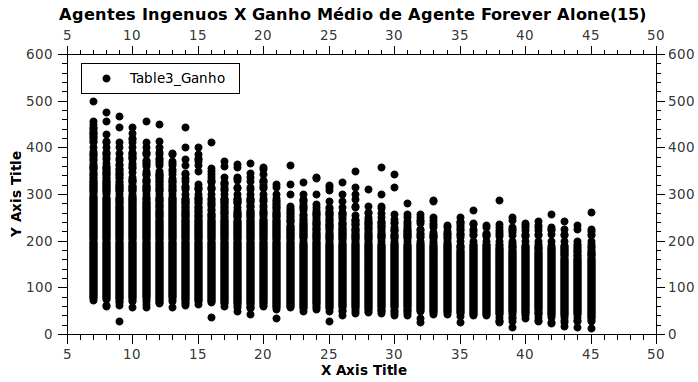
\includegraphics[scale=0.5]{Figuras/GanhoFA15.png}\\
 \scriptsize{Gráfico 5.1 - Número de agentes ingênuos X ganho médio de agente forever alone.}
\end{center}

Pode-se observar que claramente que há um descréscimo do ganho médio do agente forever alone com a introdução de mais agentes ingênuos. Isto se deve ao fato de que
a introdução deste tipo de agente não beneficia o mesmo, apenas gera concorrência.

$$$$

\begin{center}
  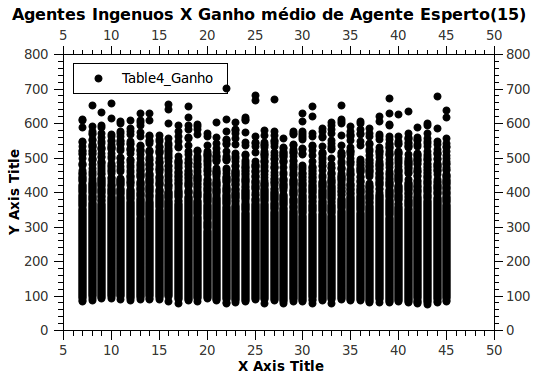
\includegraphics[scale=0.6]{Figuras/GanhoSA15.png}\\
  \scriptsize{Gráfico 5.2 - Número de agentes ingênuos X ganho médio de agente esperto.}
\end{center}

Já no gráfico 5.2 podemos observar que o ganho do agente esperto se mantém com o crescimento da população de agentes ingênuos, já que é benéfico para um agente esperto
contar com vários agentes ingênuos em sua coalisão.

$$$$

\begin{center}
   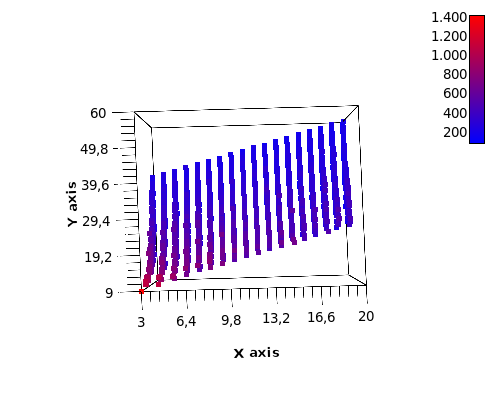
\includegraphics[scale=0.6]{Figuras/GanhoFA10(NAxNI).png}\\
  \scriptsize{Gráfico 5.3 - Número de agentes ingênuos X número total de agentes X ganho médio de agente forever alone.}
\end{center}

$$$$

\begin{center}
   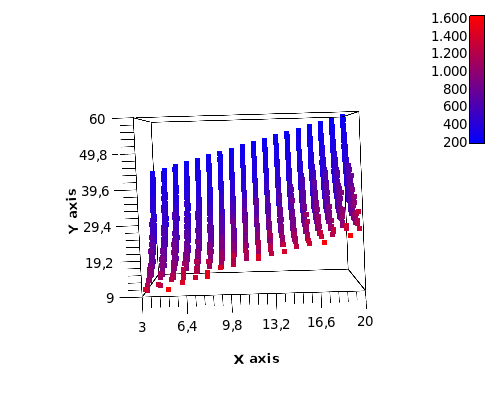
\includegraphics[scale=0.6]{Figuras/GanhoSA10(NAxNI).png}\\
  \scriptsize{Gráfico 5.3 - Número de agentes ingênuos X número total de agentes X ganho médio de agente esperto.}
\end{center}

Podemos então observar que os testes sustentam as conjecturas apresentadas.

\section{Trabalhos futuros}

\begin{enumerate}
  \item Fazer mais cargas de teste para ambientes maiores e mais agentes;
  \item Observar comportamento do ganho médio/agentes com a inclusão de insegurança (buracos, wumpus);
  \item Observar comportamento dos agentes com a possibilidade de assassinato (agentes podem matar uns aos outros).
\end{enumerate}


\begin{thebibliography}{99}

\bibitem[Russel e Norvig, 2003]{russel03} S.Russel e P. Norvig, {\em Artificial Intelligence, A Modern Approach} (2003) 197-200.

\bibitem[Wooldridge, 2009]{wooldrige09} M. Wooldridge, Forming coalitions, {\em Introduction to MultiAgent Systems} (2009), 270.

\end{thebibliography}

\end{document}




%\begin{itemize}
%\item[(a)] If $G$ is a thin spider and $R$ is empty, then
%%$dom_G[k] = dom_G[k+1] = k$, and $dom_G[j] = 0$ for every $j>k+1$.
%\[
%   dom_G[i]\ =\ 
%  \begin{cases} k, &\mbox{ if $i=k$ or $i=k+1$},\\
%                0, &\mbox{ if $i>k+1$}
%  \end{cases}
%\]
%\item[(b)] If $G$ is a thin spider and $R$ is nonempty, then
%%dom_G[k+r]=k+dom_{G[R]}[r]$ for $\chi(G[R])\leq r\leq|R|$, $dom_G[k+|R|+1]=k$, and $dom_G[j]=0$ for $j>k+|R|+1$.
%\[
%  dom_G[i]\ =\ 
%  \begin{cases} k+dom_{G[R]}[i-k], &\mbox{ if $k+\chi(G[R])\leq i\leq k+|R|$},\\
%                k,                 &\mbox{ if $i=k+|R|+1$},\\
%                0,                 &\mbox{ if $i>k+|R|+1$}
%  \end{cases}
%\]
%\item[(c)] If $G$ is a thick spider and $R$ is empty, then
%%$dom_G[k+s]=\min\{k,2k-2s\}$ for $0 \leq s\leq k$, and $dom_G[j]=0$ for $j>2k$.
%\[
%  dom_G[i]\ =\ 
%  \begin{cases} \min\{k,4k-2i\}, &\mbox{ if $k\leq i\leq 2k$},\\
%                0,               &\mbox{ if $i>2k$}
%  \end{cases}
%\]
%\item[(d)] If $G$ is a thick spider and $R$ is nonempty, then
%%$dom_G[k+r]=k+dom_{G[R]}[r]$ for $\chi(G[R])\leq r\leq|R|$, $dom_G[k+|R|+s]=\min\{k,2k-2s\}$, for $1\leq s\leq k$, and $dom_G[j]=0$ for $j>2k+|R|$.
%\[
%  dom_G[i]\ =\ 
%  \begin{cases} k+dom_{G[R]}[i-k],    &\mbox{ if $k+\chi(G[R])\leq i\leq k+|R|$},\\
%                \min\{k,4k-2i+2|R|\}, &\mbox{ if $k+|R|+1\leq i\leq 2k+|R|$},\\
%                0,                    &\mbox{ if $i>2k+|R|$}
%  \end{cases}
%\]
%\end{itemize}
